\documentclass[../main.tex]{subfiles}
\graphicspath{{\subfix{..}}}
\begin{document}
\begin{appendices}
\section{Exploratory Data Analysis}
\begin{table}[H]
	\centering
	\caption{Bandwidths translation between Sentinel2 and the datasets \cite{sen12mscr} \& \cite{sen12mscrts}.}
	
	\begin{tabular}{llr}
		\hline
		Band Sentinel2 & Name                & Band ID \\ \hline
		B1             & Coastal aerosol     &       0 \\
		B2             & Blue                &       1 \\
		B3             & Green               &       2 \\
		B4             & Red                 &       3 \\
		B5             & Vegetation Red Edge &       4 \\
		B6             & Vegetation Red Edge &       5 \\
		B7             & Vegetation Red Edge &       6 \\
		B8             & NIR                 &       7 \\
		B8A            & Vegetation Red Edge &       8 \\
		B9             & Water Vapour        &       9 \\
		B10            & SWIR-Cirrus         &      10 \\
		B11            & SWIR                &      11 \\
		B12            & SWIR                &      12 \\ \hline
	\end{tabular}
	\label{tab:band-translation}
\end{table}
\begin{figure}[H]
	\centering
	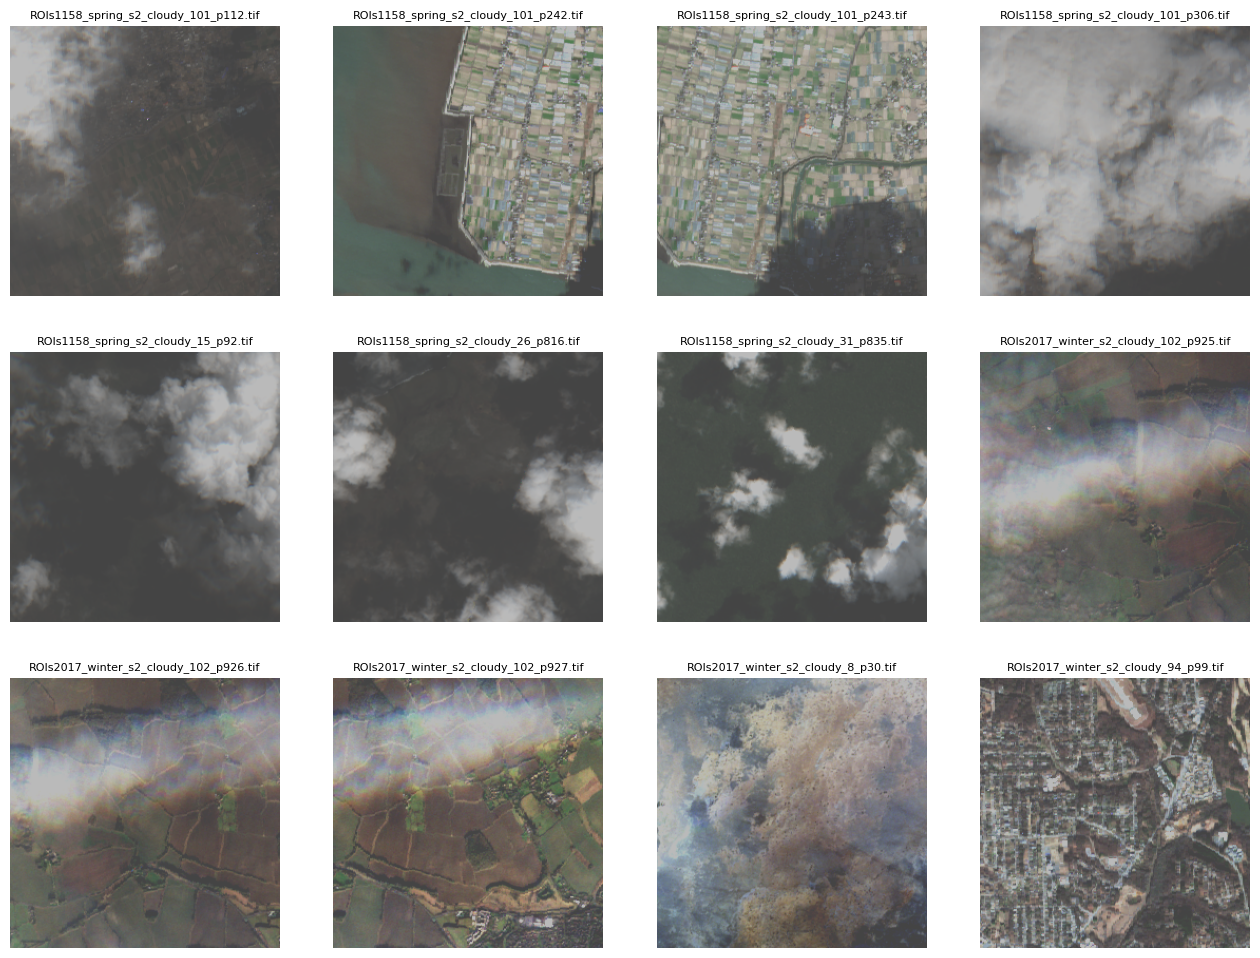
\includegraphics[width=16cm]{imgs/eda/first-visualization}
	\caption{12 images of the sample showing the diversity of cloudy images.}
	\label{fig:eda-first-exploration}
\end{figure}
\begin{figure}[H]
	\centering
	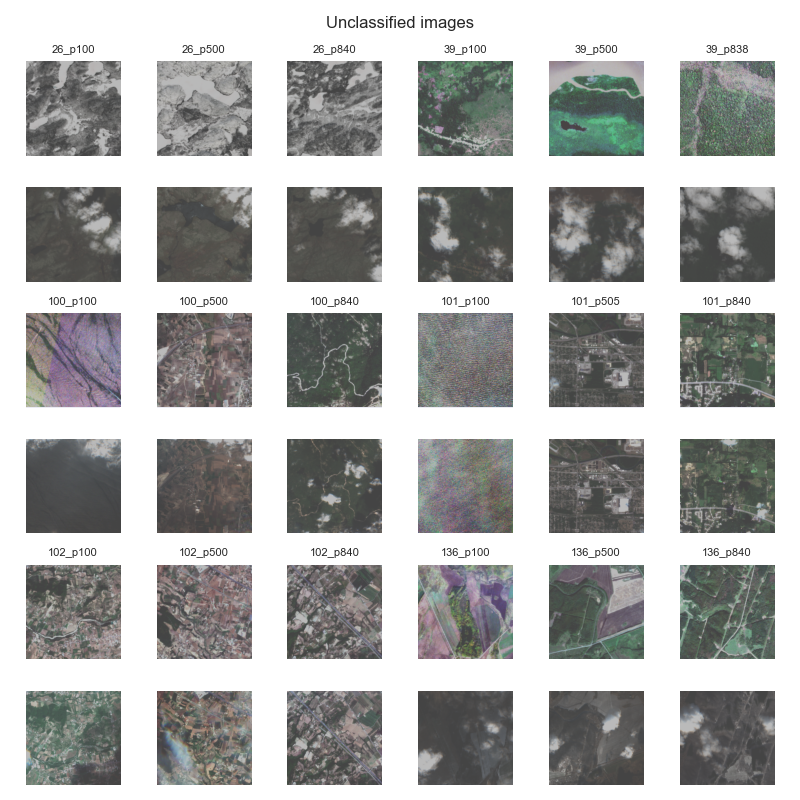
\includegraphics[width=16cm]{imgs/eda/unclassified}
	\caption{Unclassified images}
	\label{fig:eda-unclassified}
\end{figure}
\begin{figure}[H]
	\centering
	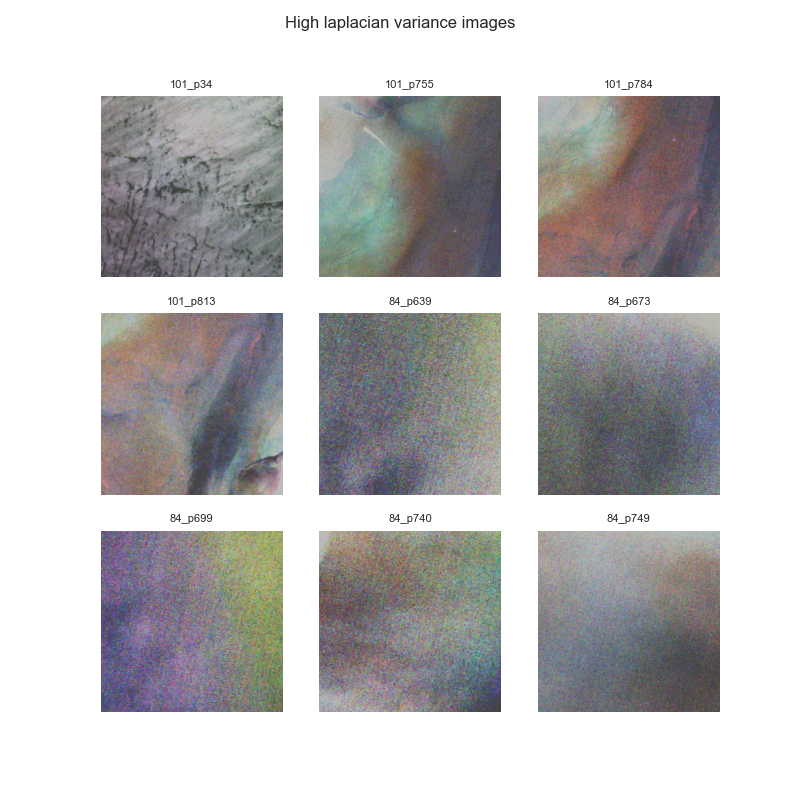
\includegraphics[width=16cm]{imgs/eda/high-blur}
	\caption{Sample of images with high laplacian variance, blurriness.}
	\label{fig:eda-blurriness-images}
\end{figure} 
\begin{figure}[H]
	\centering
	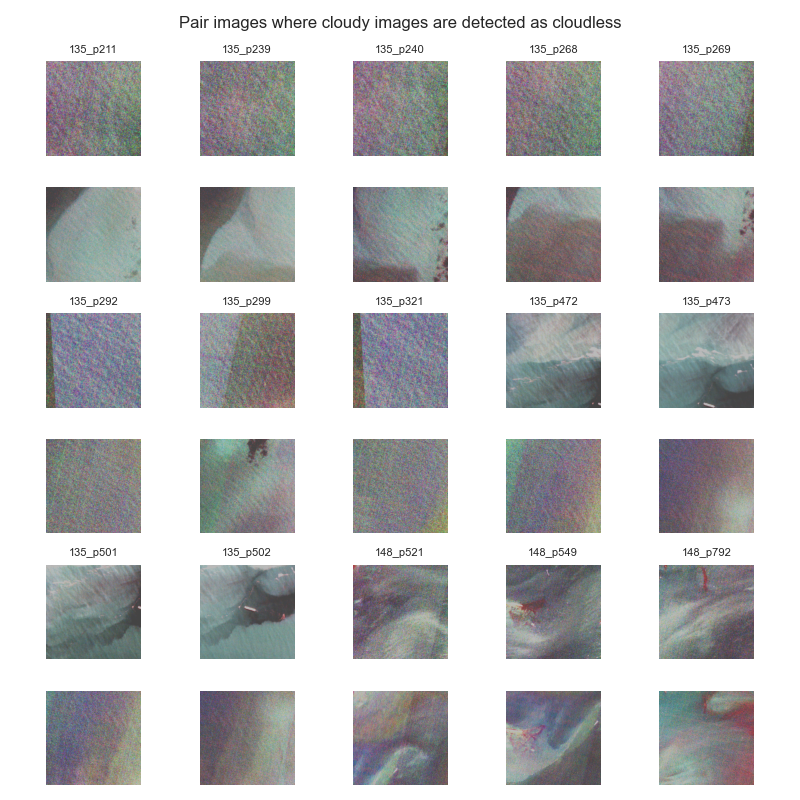
\includegraphics[width=16cm]{imgs/eda/cloudly-but-cloudless}
	\caption{Sample of images labeled as cloudy but with low cloud cover percentage area.}
	\label{fig:eda-low-cloud-but-cloudy}
\end{figure} 
\begin{figure}[H]
	\centering
	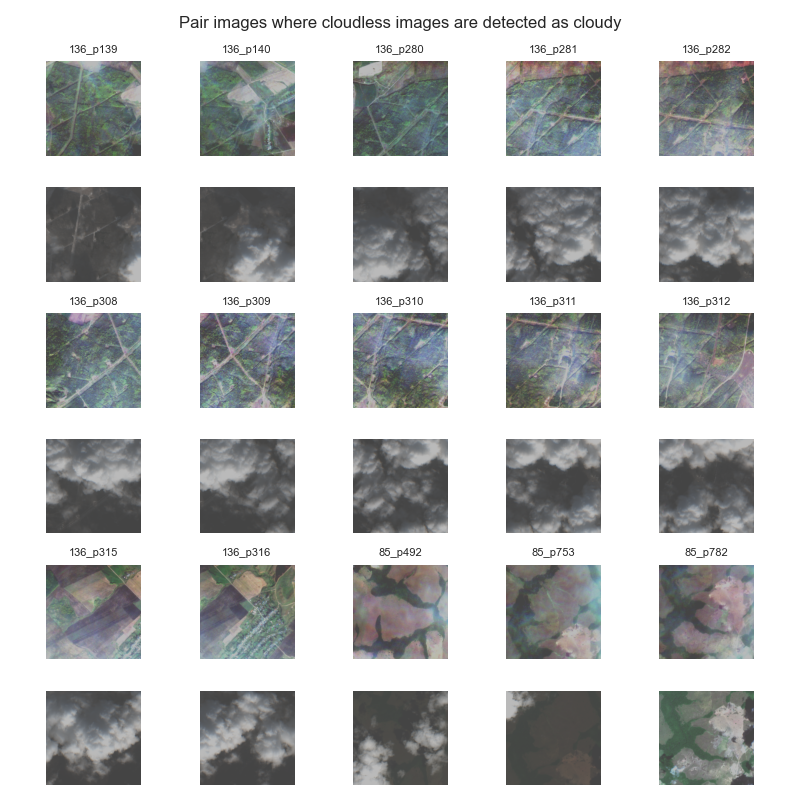
\includegraphics[width=16cm]{imgs/eda/cloudless-but-cloudy}
	\caption{Sample of images labeled as cloudy but with low cloud cover percentage area.}
	\label{fig:eda-haze-cloudless}
\end{figure}
	\begin{figure}[H]
	\centering
	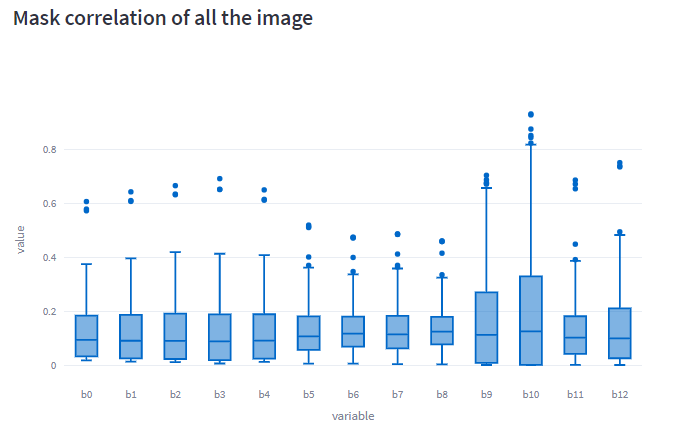
\includegraphics[width=13cm]{imgs/eda/mask-correlation}
	\caption{Correlation of the image and the values of the band, by mean from each image.}
	\label{fig:eda-mask-correlation-b10}
\end{figure}
	\begin{figure}[H]
	\centering
	\begin{subfigure}[b]{0.85\textwidth}
		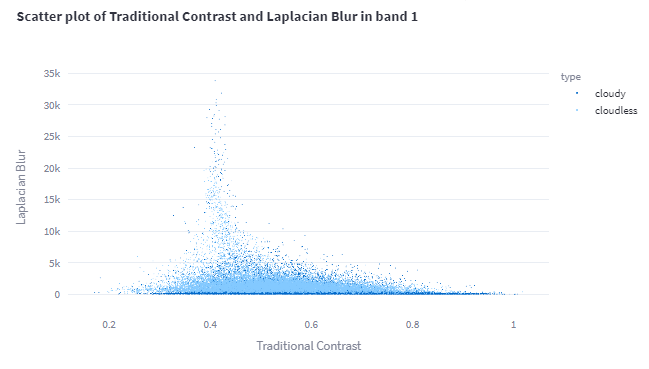
\includegraphics[width=\textwidth]{imgs/eda/b1-contrast-blurriness}	
		\caption{Scatter plot of the contrast and the laplacian variance of B1}	
	\end{subfigure}
	\begin{subfigure}[b]{0.85\textwidth}
		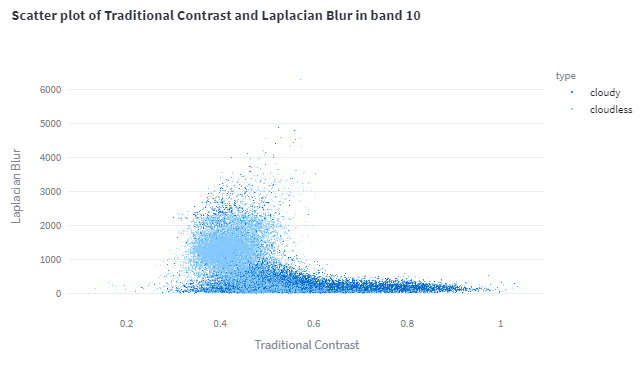
\includegraphics[width=\textwidth]{imgs/eda/b10-contrast-blurriness}	
		\caption{Scatter plot of the contrast and the laplacian variance of B10}		
	\end{subfigure}
	\caption{Comparison between B1 and B10 regarding blurriness and contrast.}
	\label{fig:eda-comparison-b1-b10}
\end{figure}
\begin{figure}[H]
	\centering
	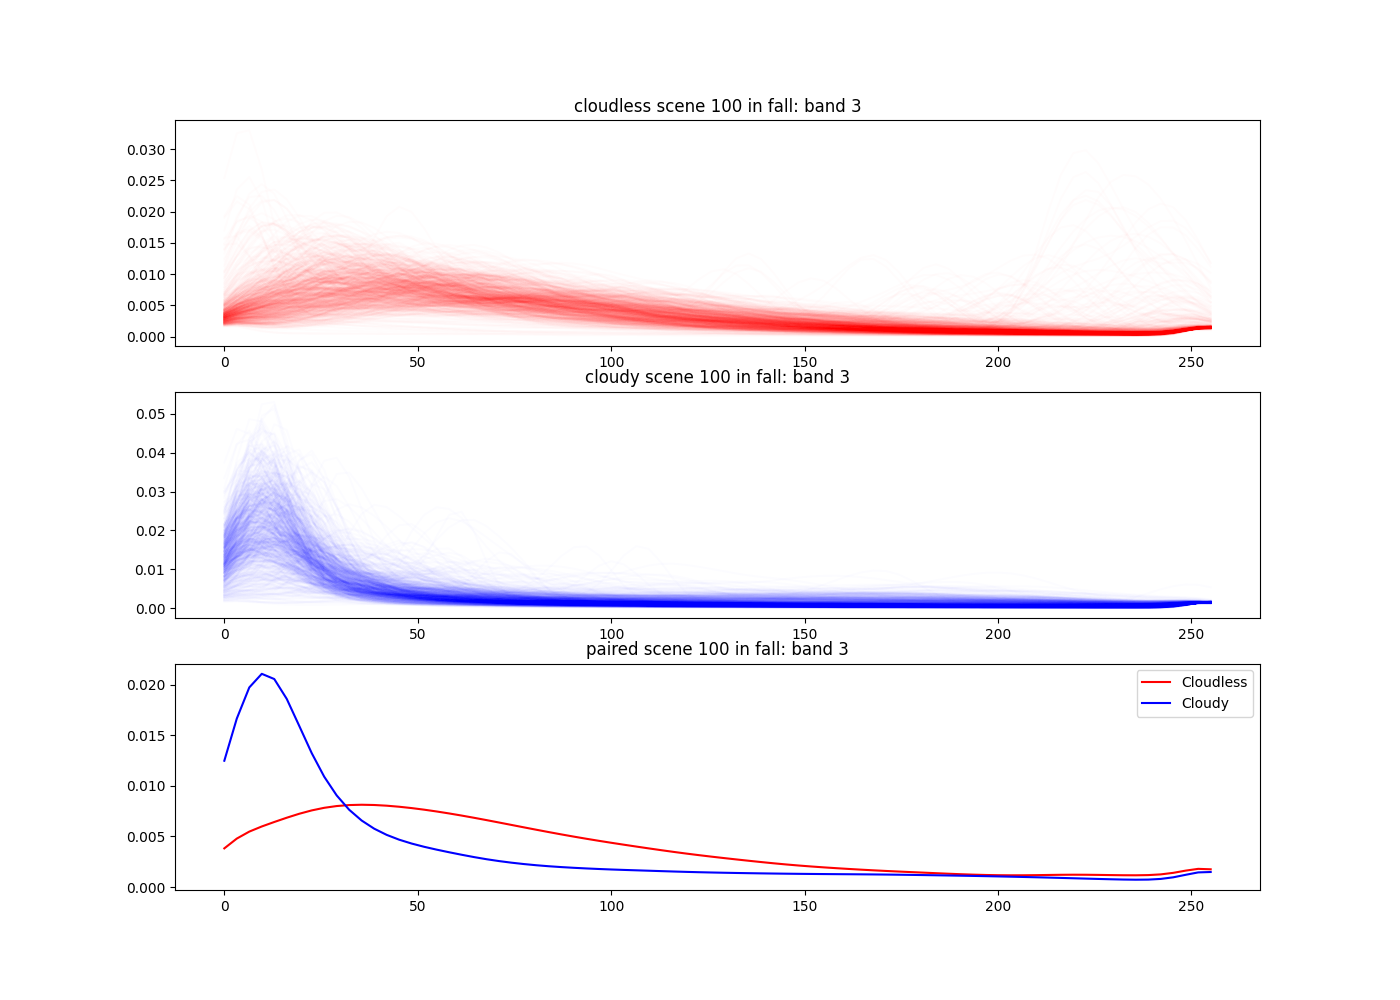
\includegraphics[width=16cm]{imgs/eda/b3-kde}
	\caption{Kernel density estimation of B3 in cloudy and cloudless the patches of a specific scene (100)}
	\label{fig:eda-b3-kde}
\end{figure}
\begin{figure}[H]
	\centering
	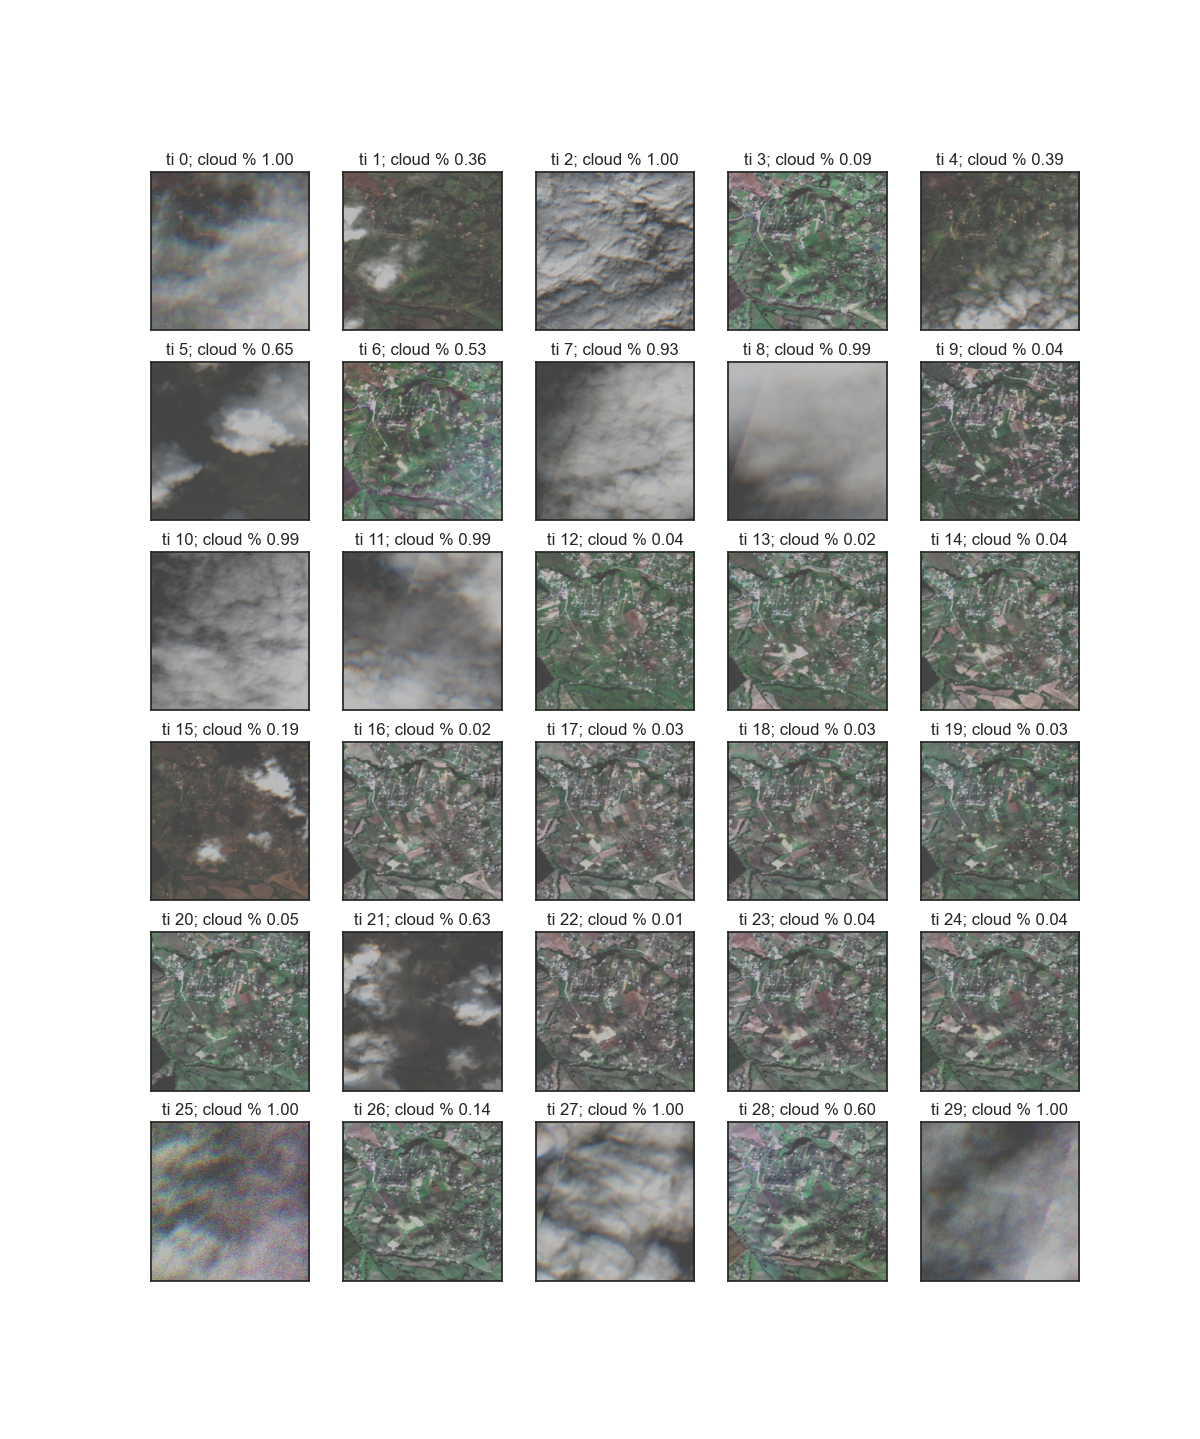
\includegraphics[width=16cm]{imgs/eda/merge/cloud-percentages-patch-images}
	\caption{Patch exploration in all intervals.}
	\label{fig:eda-merge-patch-xploration}
\end{figure}
\begin{figure}[H]
	\centering
	\enlargethispage{5cm}
	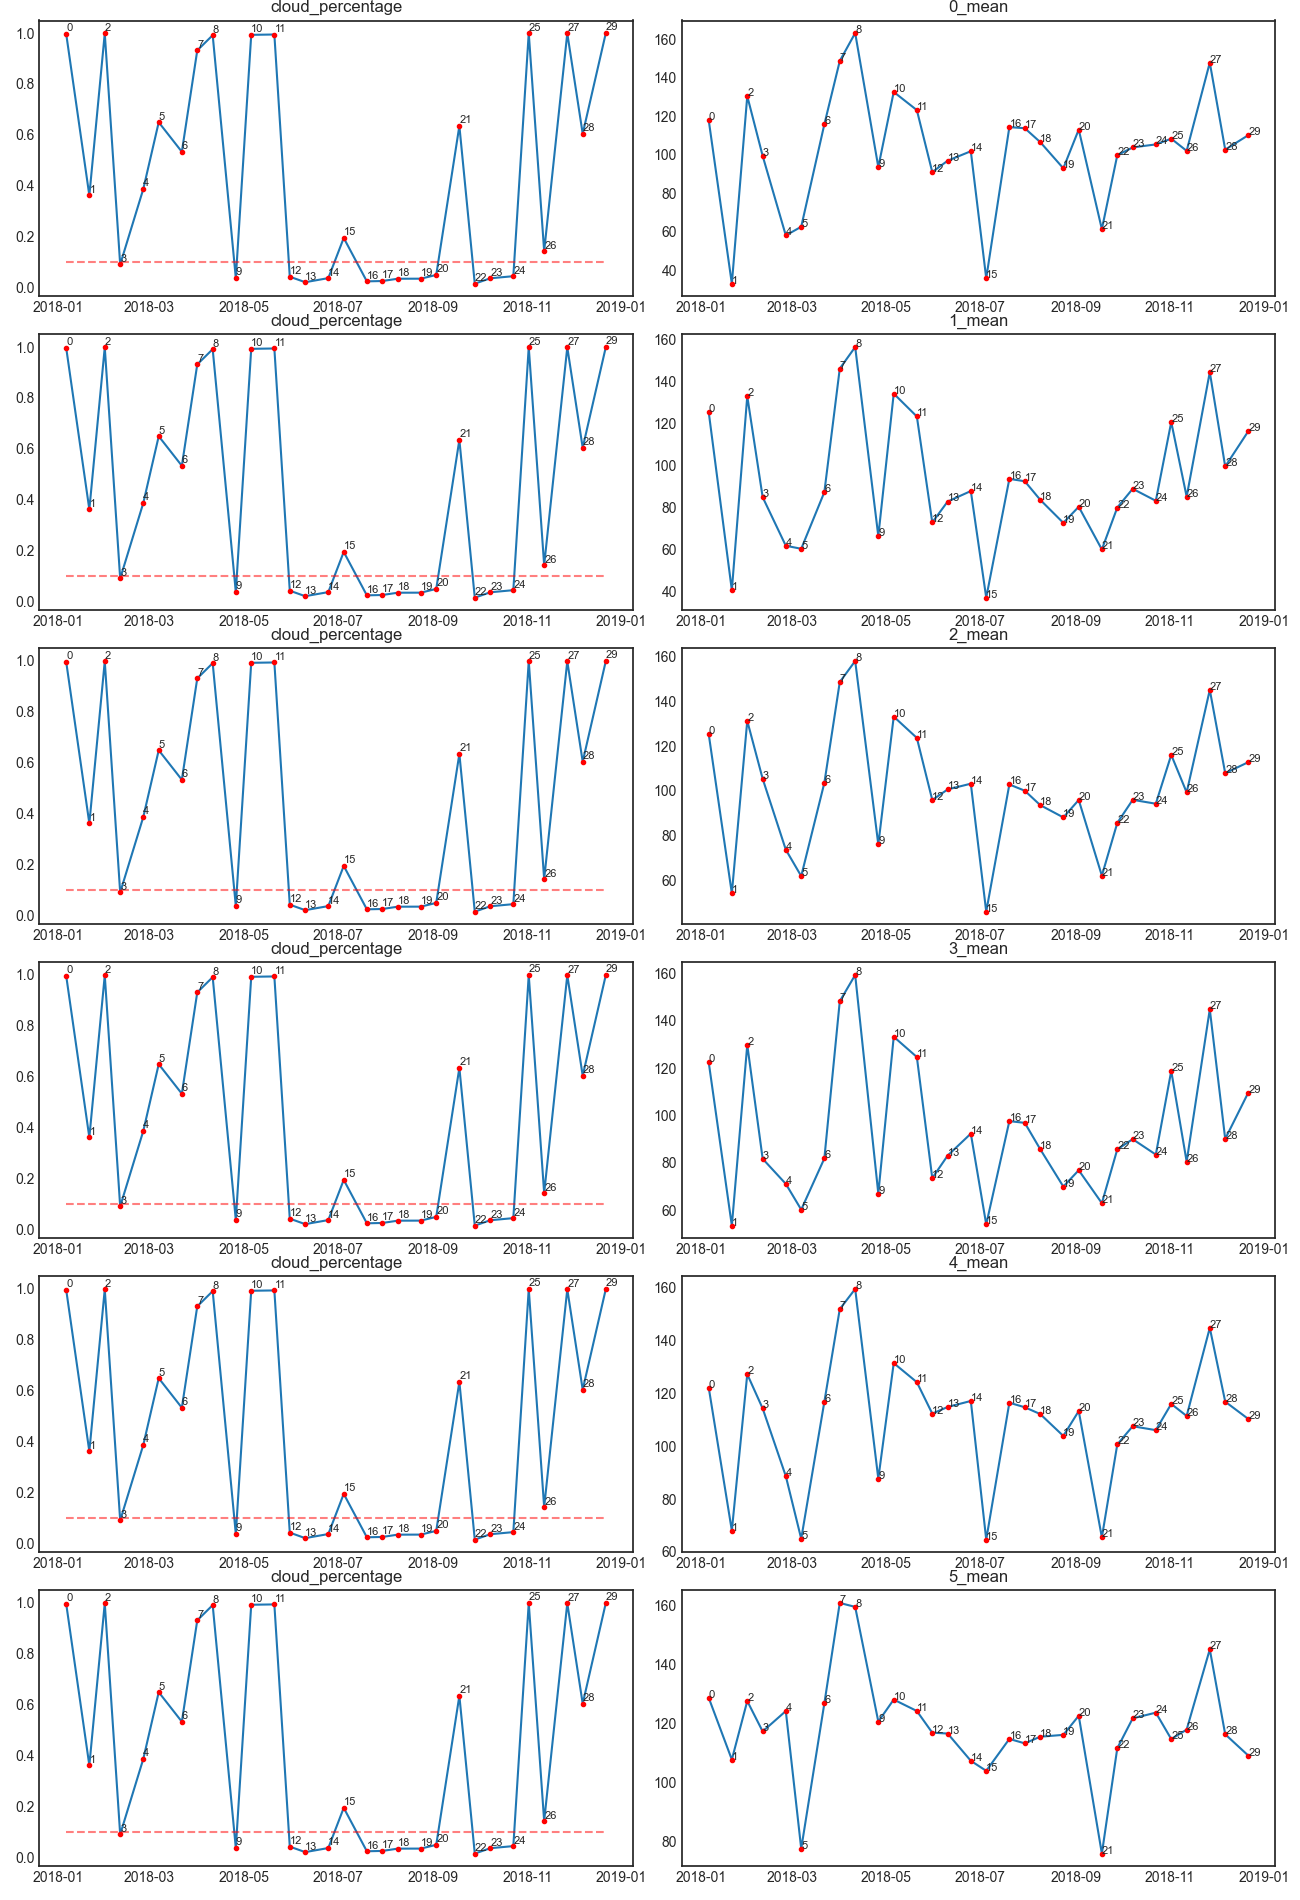
\includegraphics[width=15cm]{imgs/eda/merge/cloud-percentage-each-time-interval-band-1}
	\caption{Cloud percentage and band mean value in all time instances (1).}
	\label{fig:eda-merge-patch-xploration-band-1}
\end{figure}
\begin{figure}[H]
	\centering
	\enlargethispage{5cm}
	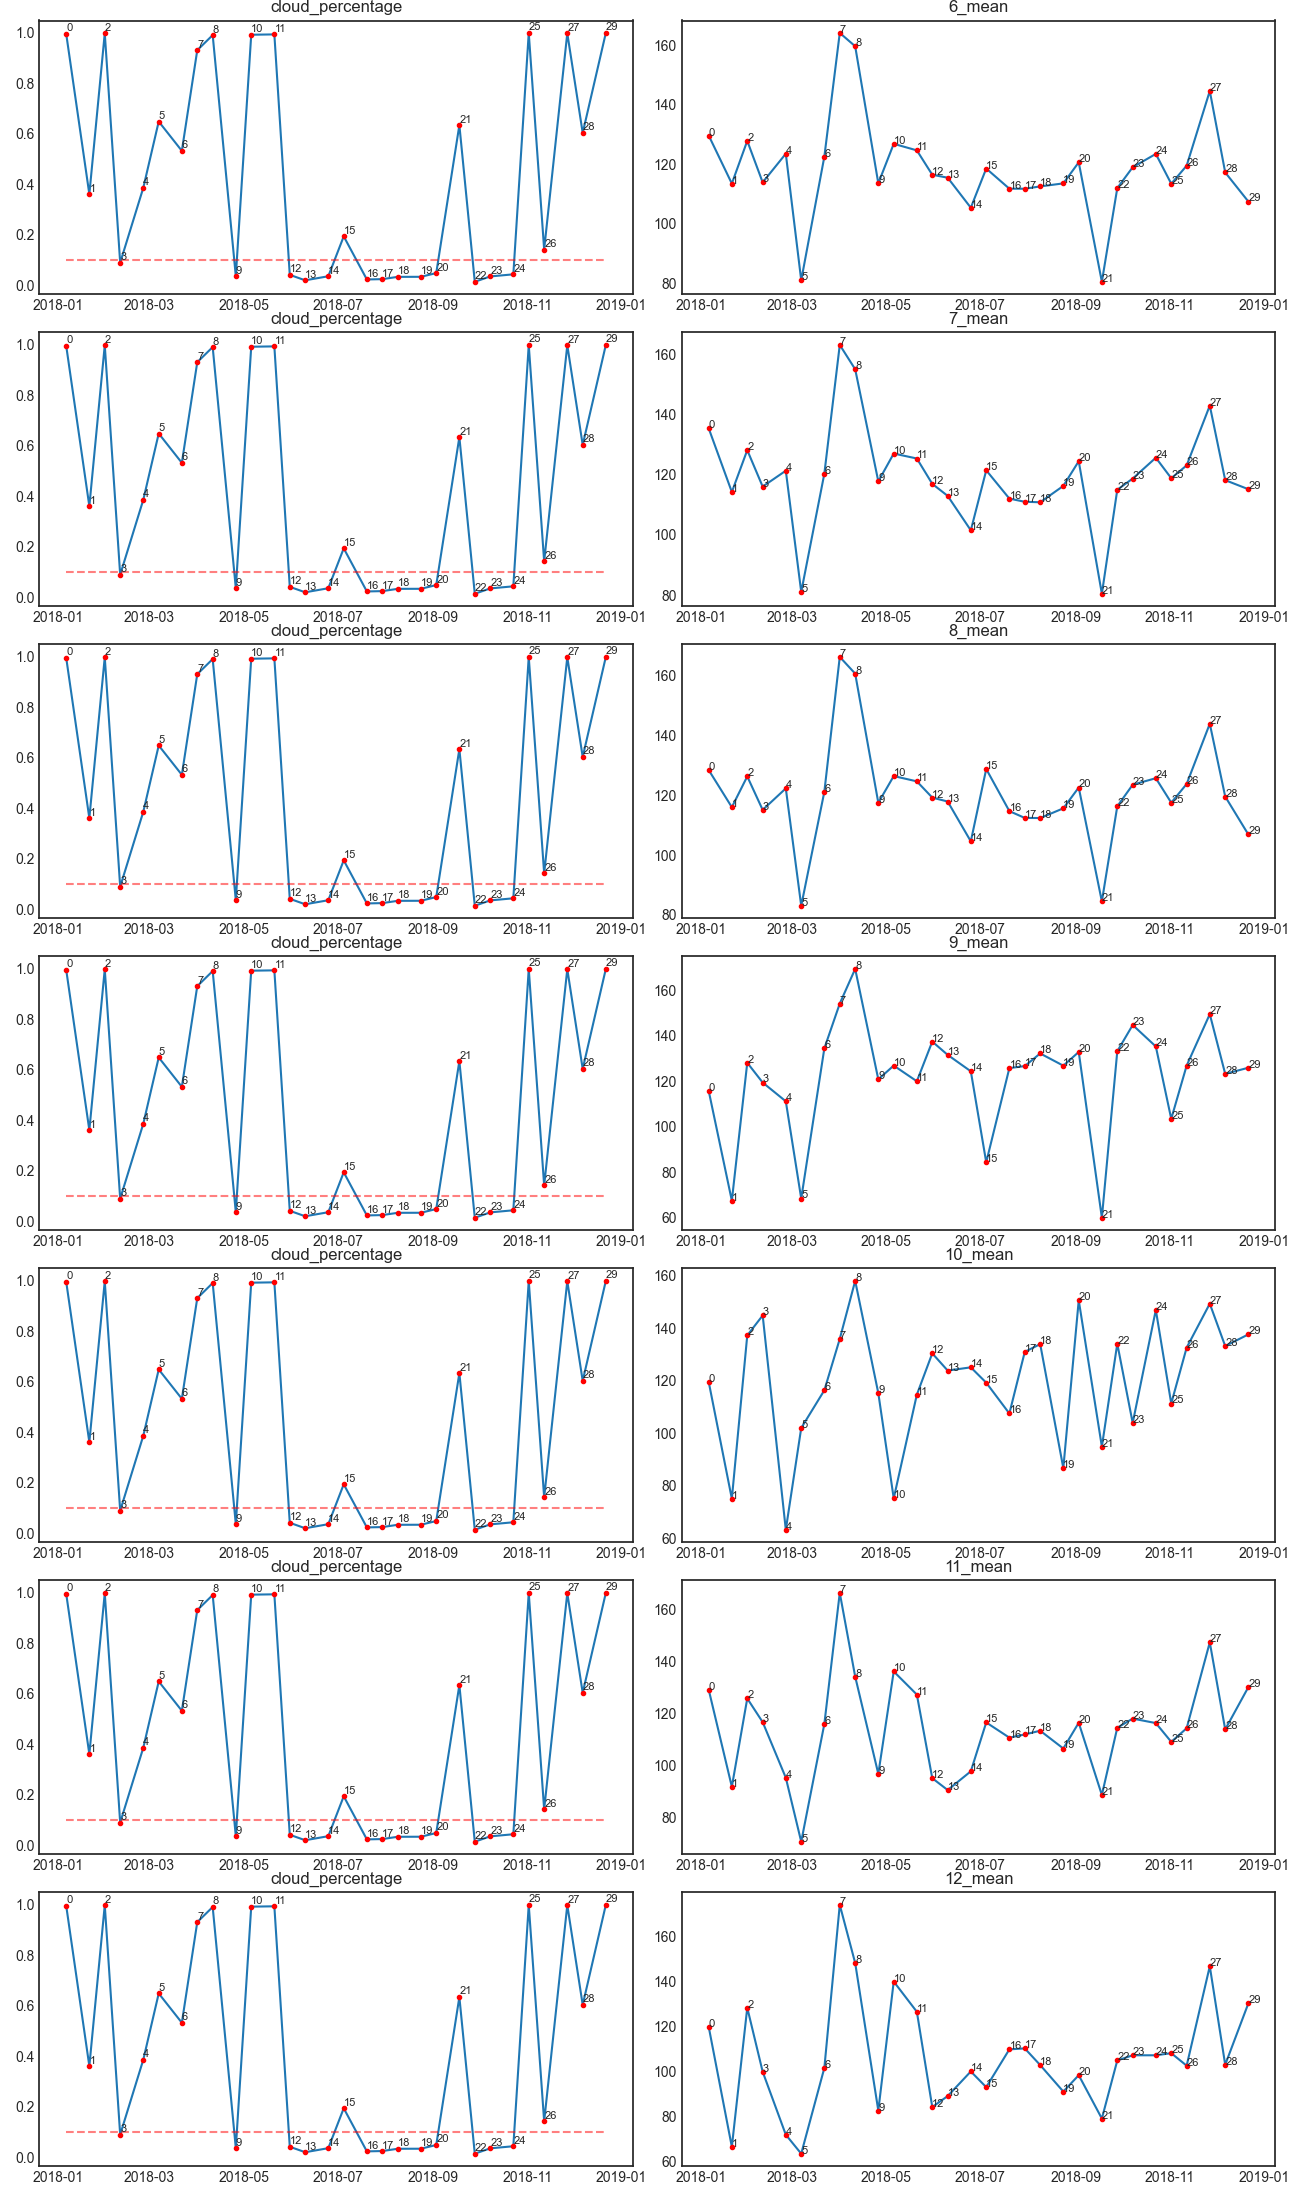
\includegraphics[width=15cm]{imgs/eda/merge/cloud-percentage-each-time-interval-band-2}
	\caption{Cloud percentage and band mean value in all time instances (2).}
	\label{fig:eda-merge-patch-xploration-band-2}
\end{figure}
\begin{figure}[H]
	\centering
	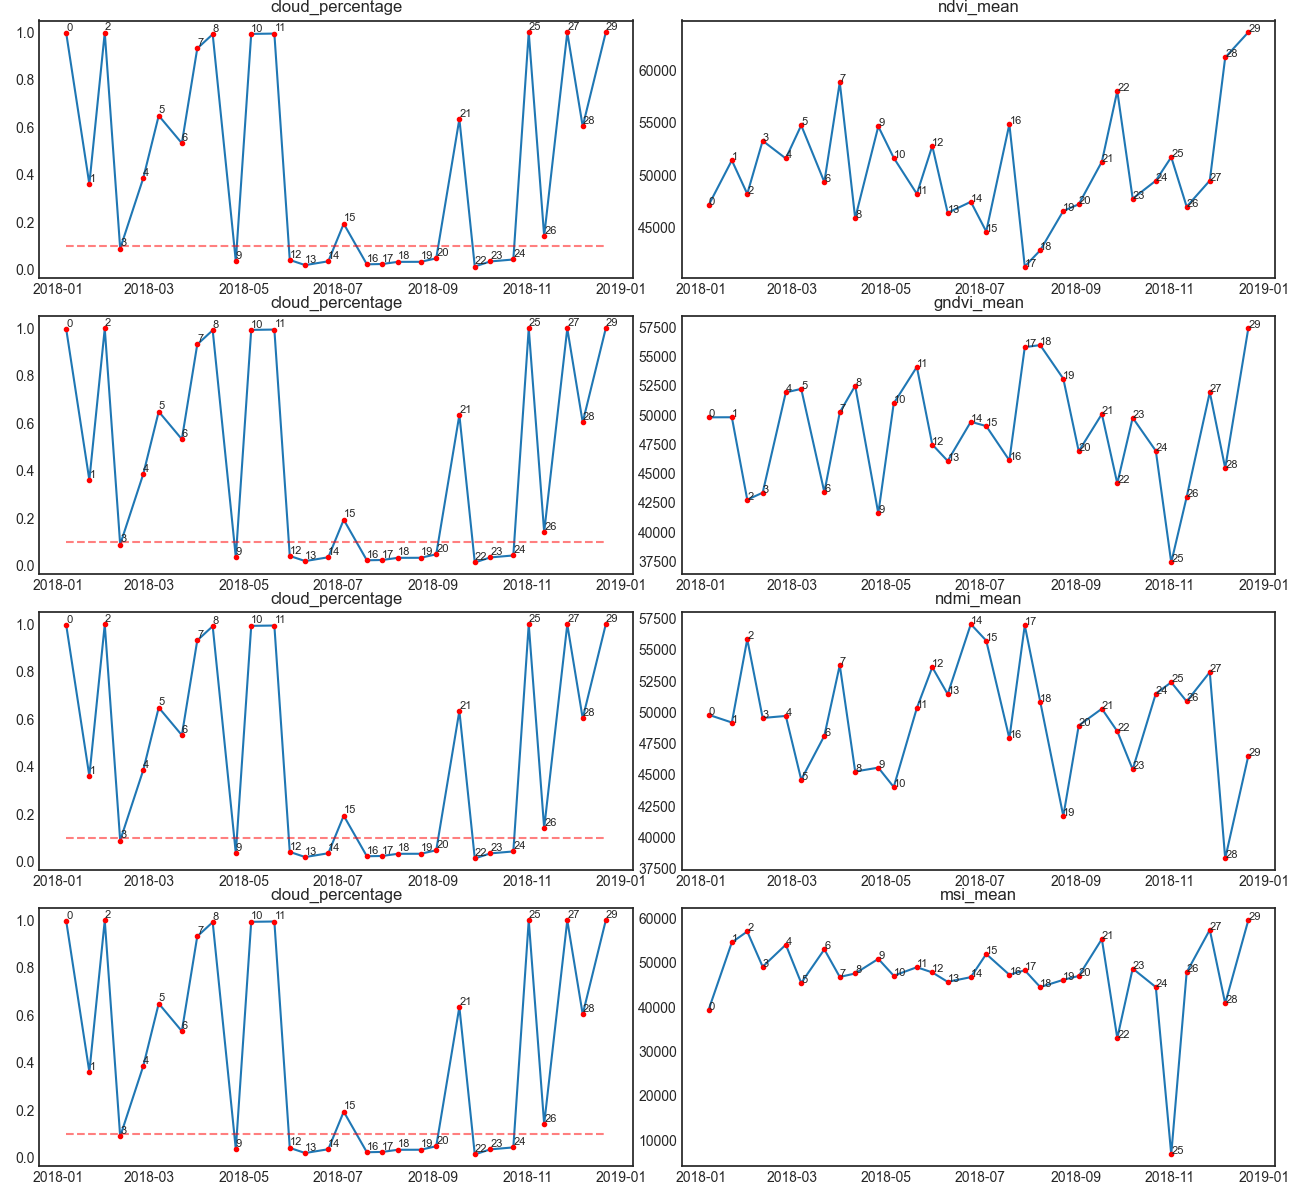
\includegraphics[width=15cm]{imgs/eda/merge/cloud-percentage-each-time-interval-index-1}
	\caption{Cloud percentage and index mean value in all time instances (1).}
	\label{fig:eda-merge-patch-xploration-index-1}
\end{figure}
\begin{figure}[H]
	\centering
	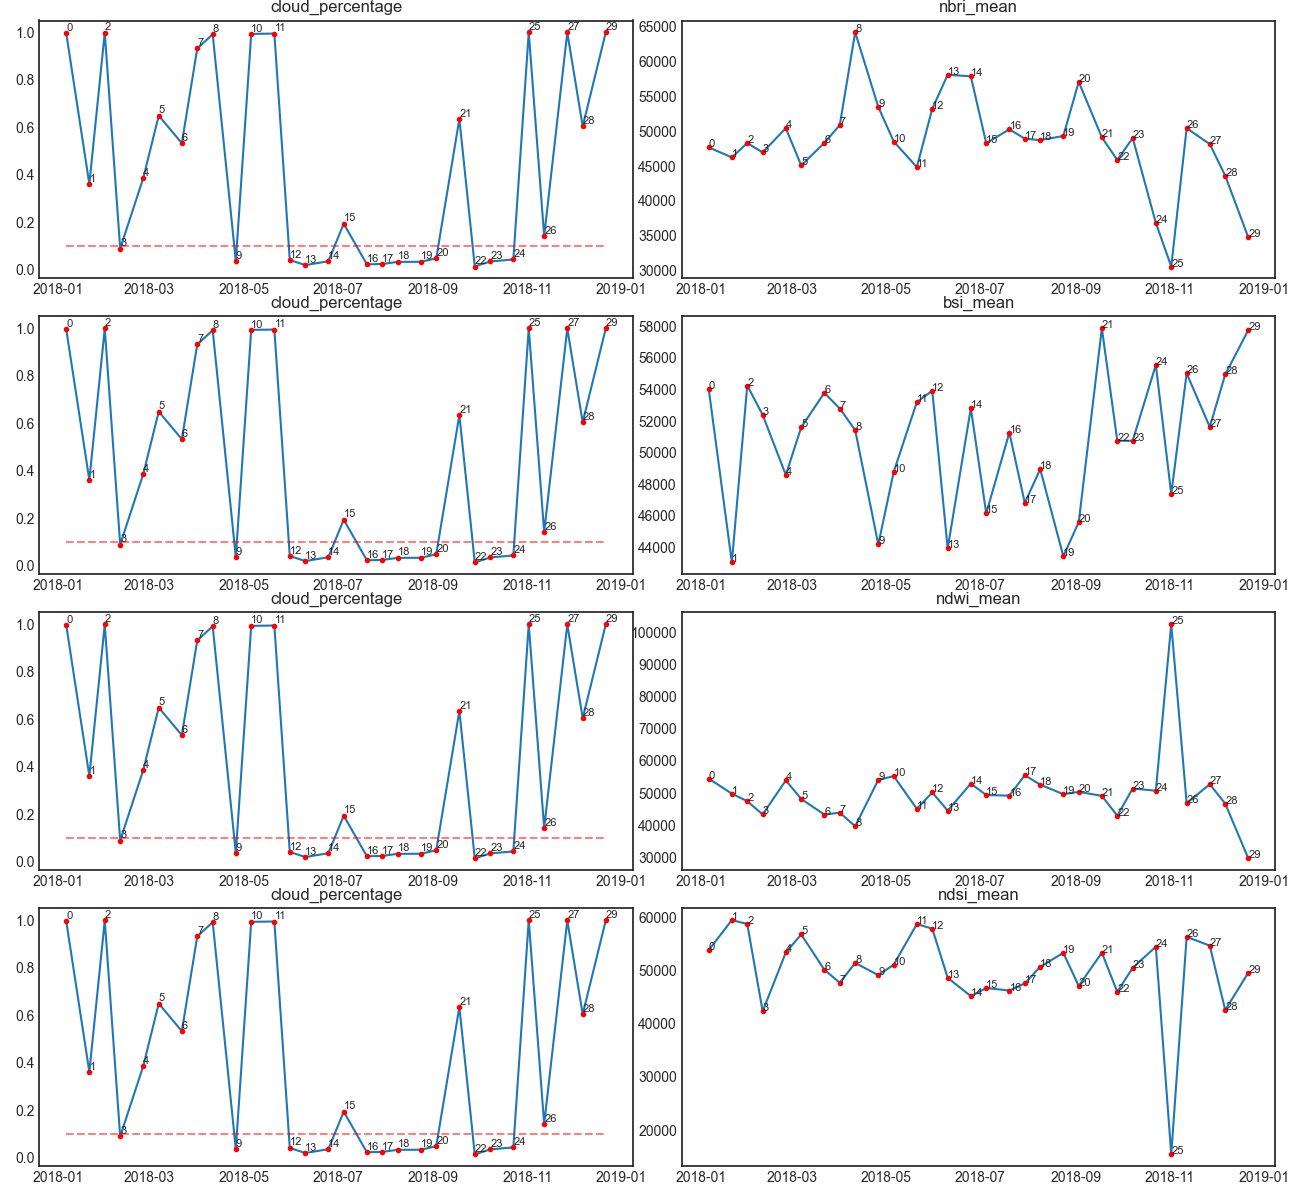
\includegraphics[width=15cm]{imgs/eda/merge/cloud-percentage-each-time-interval-index-2}
	\caption{Cloud percentage and index mean value in all time instances (2).}
	\label{fig:eda-merge-patch-xploration-index-1}
\end{figure}
\end{appendices}
\end{document}